
\subsection{Resultats}

A continuació es recullen els mapes de temperatura de l'anàlisi de densitat de malla, de pas de temps i de l'esquema d'integracia temporal.

\begin{figure}[ht]
	\centering
	\begin{subfigure}{.5\textwidth}
		\centering
		\includegraphics[width=.95\linewidth]{imagenes/04_analisi_influencia_dades_numeriques/malla/malla_1.pdf}
		\vspace{-15pt}
		\caption{Temps $t_\text{max} = 5000 \ \second$, discretització $N_1 = 5$.}
		\label{fig:malla_1}
	\end{subfigure}%
	\begin{subfigure}{.5\textwidth}
		\centering
		\includegraphics[width=.95\linewidth]{imagenes/04_analisi_influencia_dades_numeriques/malla/malla_2.pdf}
		\vspace{-15pt}
		\caption{Temps $t_\text{max} = 5000 \ \second$, discretització $N_1 = 15$.}
		\label{fig:malla_2}
	\end{subfigure}
	\begin{subfigure}{.5\textwidth}
		\centering
		\includegraphics[width=.95\linewidth]{imagenes/04_analisi_influencia_dades_numeriques/malla/malla_3.pdf}
		\vspace{-15pt}
		\caption{Temps $t_\text{max} = 5000 \ \second$, discretització $N_1 = 25$.}
		\label{fig:malla_3}
	\end{subfigure}%
	\begin{subfigure}{.5\textwidth}
		\centering
		\includegraphics[width=.95\linewidth]{imagenes/04_analisi_influencia_dades_numeriques/malla/malla_4.pdf}
		\vspace{-15pt}
		\caption{Temps $t_\text{max} = 5000 \ \second$, discretització $N_1 = 35$.}
		\label{fig:malla_4}
	\end{subfigure}
	\begin{subfigure}{.5\textwidth}
		\centering
		\includegraphics[width=.95\linewidth]{imagenes/04_analisi_influencia_dades_numeriques/malla/malla_5.pdf}
		\vspace{-15pt}
		\caption{Temps $t_\text{max} = 5000 \ \second$, discretització $N_1 = 45$.}
		\label{fig:malla_5}
	\end{subfigure}%
	\begin{subfigure}{.5\textwidth}
		\centering
		\includegraphics[width=.95\linewidth]{imagenes/04_analisi_influencia_dades_numeriques/malla/malla_6.pdf}
		\vspace{-15pt}
		\caption{Temps $t_\text{max} = 5000 \ \second$, discretització $N_1 = 55$.}
		\label{Temps fig:malla_6}
	\end{subfigure}
	\caption{(Anàlisi de la densitat de malla) Mapes de temperatures en $t_\text{max} = 5000 \ \second$, discretitzacions uniformes de $N_1 = 5, \, 15, \, 25, \, 35, \, 45$ i $55$ nodes, pas de temps $\Delta = 1.00 \ \second$, esquema Crank--Nicolson i sense interpolació. L'escala de temperatures és entre $20 \ \celsius$ i $40 \ \celsius$. Els materials amb temperatures més uniformes són $M1$ i $M3$. En aquests, la diferència entre discretitzacions espacials no és significativa. La zona amb un major gradient de temperatures és la paret dreta i la cantonada inferior dreta a causa de les condicions de contorn. En aquestes regions la millora en densificar la malla és notable. La discretització amb $N_1 = 45$ té $4582$ nodes, mentre que la discretització amb $N_1 = 55$ en té $7474$, la qual cosa incrementa el temps de càlcul. Com s'aprecia, la diferència entre ambdues discretitzacions en la regió amb major gradient tèrmic és petita.}
	\label{fig:malla_5000}
\end{figure} 

\begin{figure}[ht]
	\centering
	\begin{subfigure}{.5\textwidth}
		\centering
		\includegraphics[width=.95\linewidth]{imagenes/04_analisi_influencia_dades_numeriques/malla/malla_7.pdf}
		\vspace{-15pt}
		\caption{Temps $t_\text{max} = 10000 \ \second$, discretització $N_1 = 5$.}
		\label{fig:malla_7}
	\end{subfigure}%
	\begin{subfigure}{.5\textwidth}
		\centering
		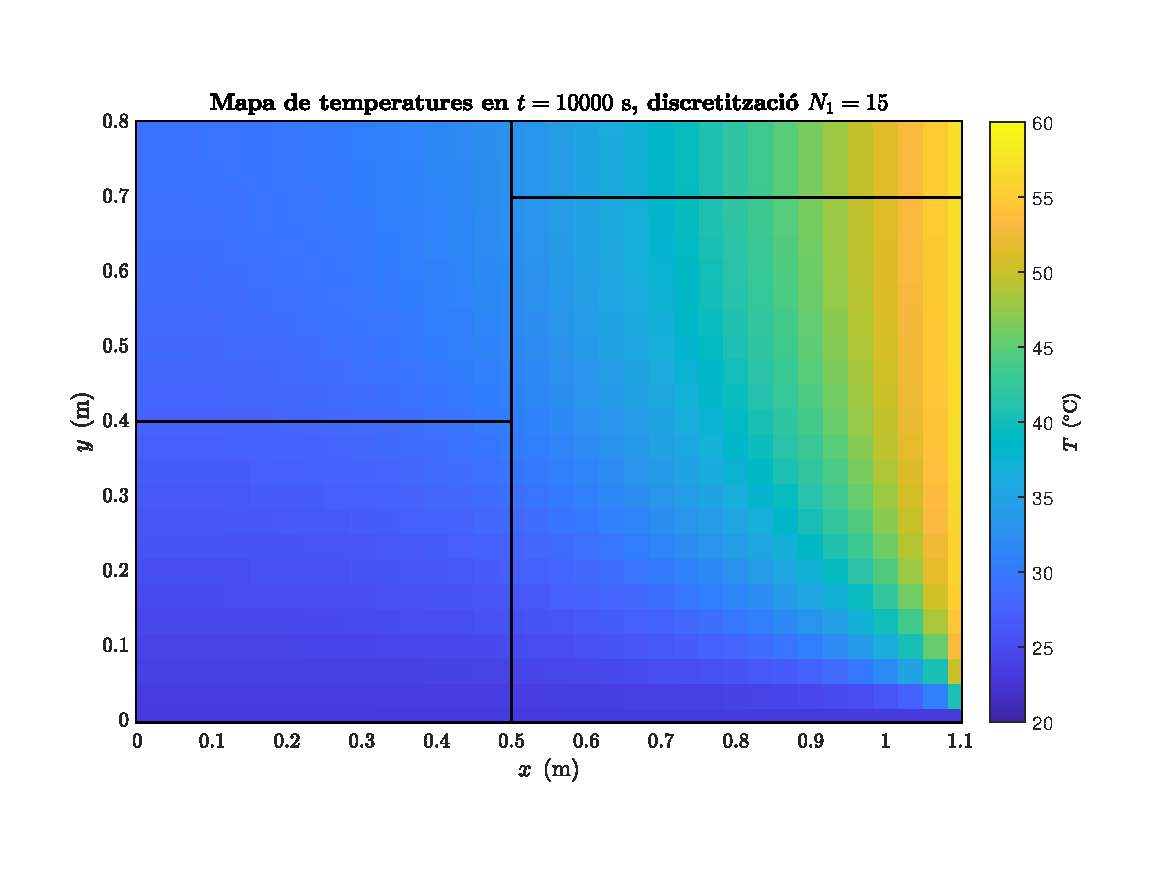
\includegraphics[width=.95\linewidth]{imagenes/04_analisi_influencia_dades_numeriques/malla/malla_8.pdf}
		\vspace{-15pt}
		\caption{Temps $t_\text{max} = 10000 \ \second$, discretització $N_1 = 15$.}
		\label{fig:malla_8}
	\end{subfigure}
	\begin{subfigure}{.5\textwidth}
		\centering
		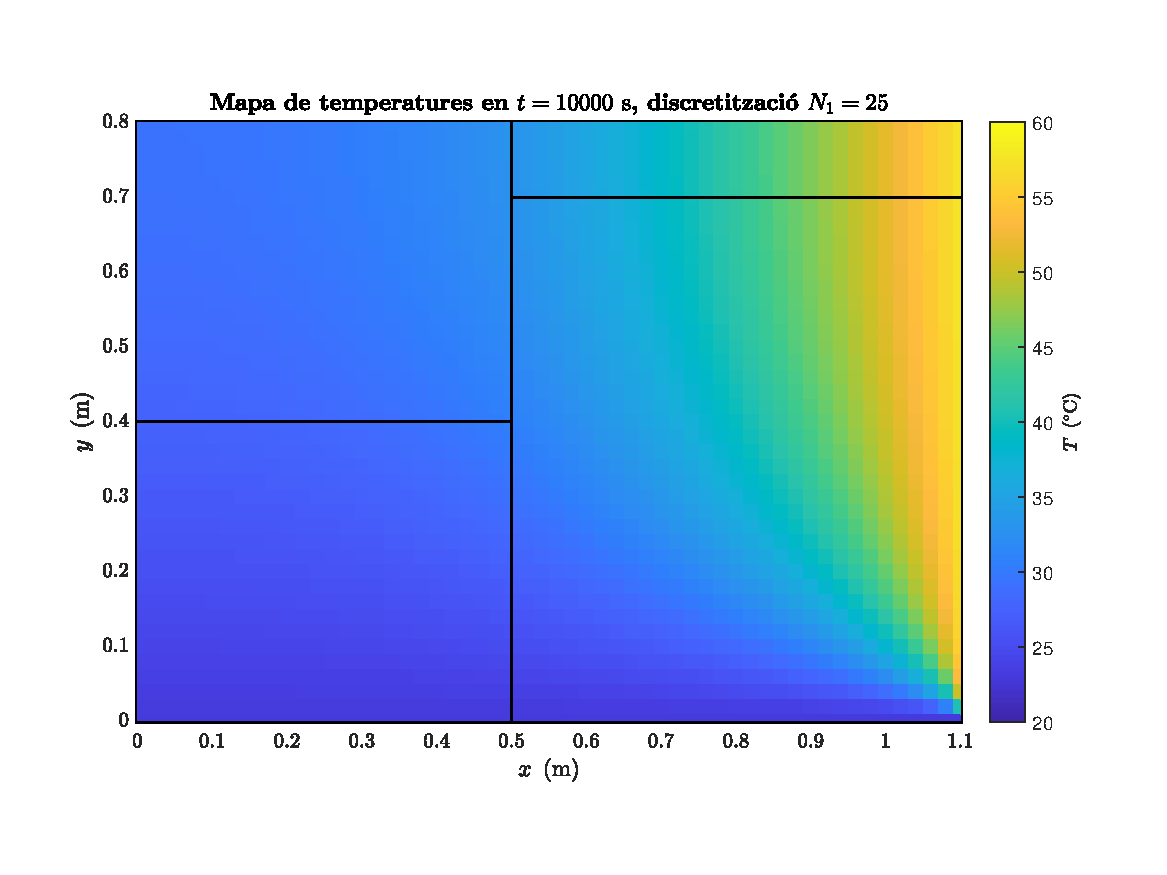
\includegraphics[width=.95\linewidth]{imagenes/04_analisi_influencia_dades_numeriques/malla/malla_9.pdf}
		\vspace{-15pt}
		\caption{Temps $t_\text{max} = 10000 \ \second$, discretització $N_1 = 25$.}
		\label{fig:malla_9}
	\end{subfigure}%
	\begin{subfigure}{.5\textwidth}
		\centering
		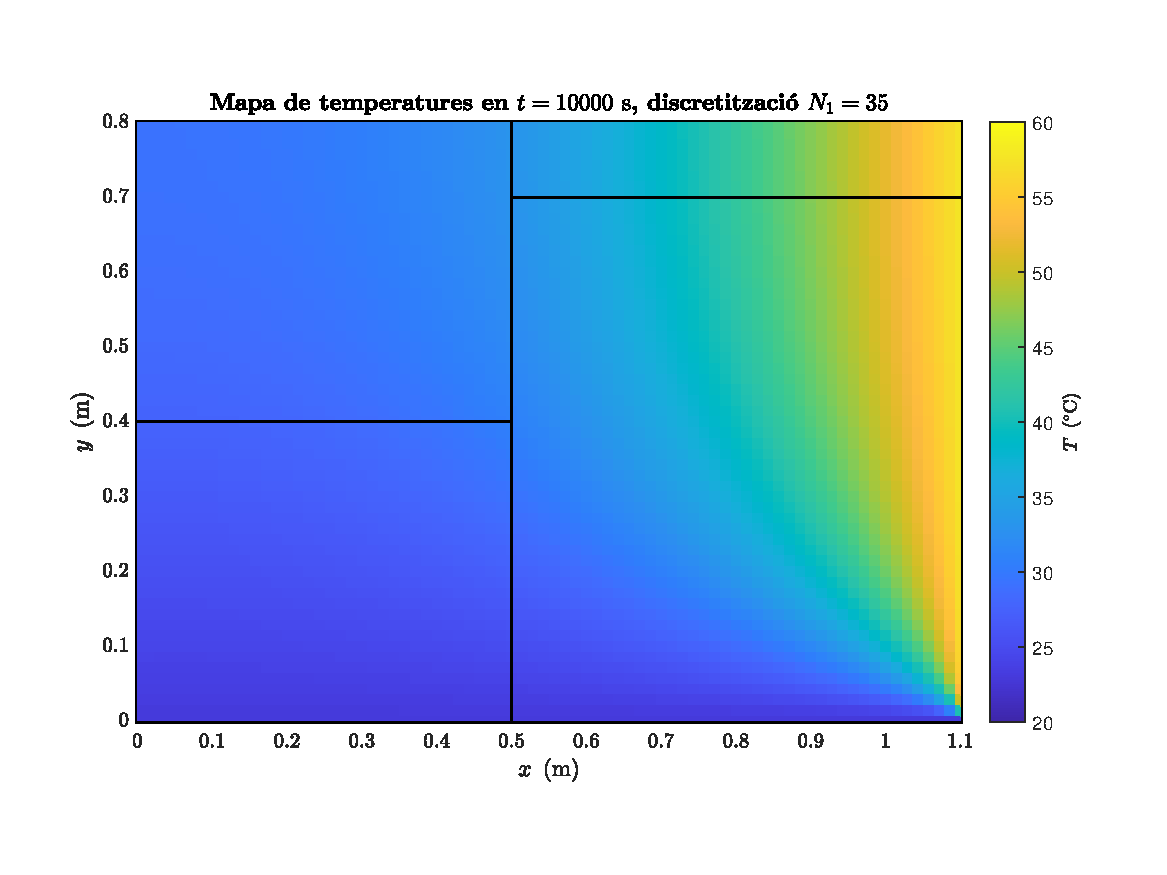
\includegraphics[width=.95\linewidth]{imagenes/04_analisi_influencia_dades_numeriques/malla/malla_10.pdf}
		\vspace{-15pt}
		\caption{Temps $t_\text{max} = 10000 \ \second$, discretització $N_1 = 35$.}
		\label{fig:malla_10}
	\end{subfigure}
	\begin{subfigure}{.5\textwidth}
		\centering
		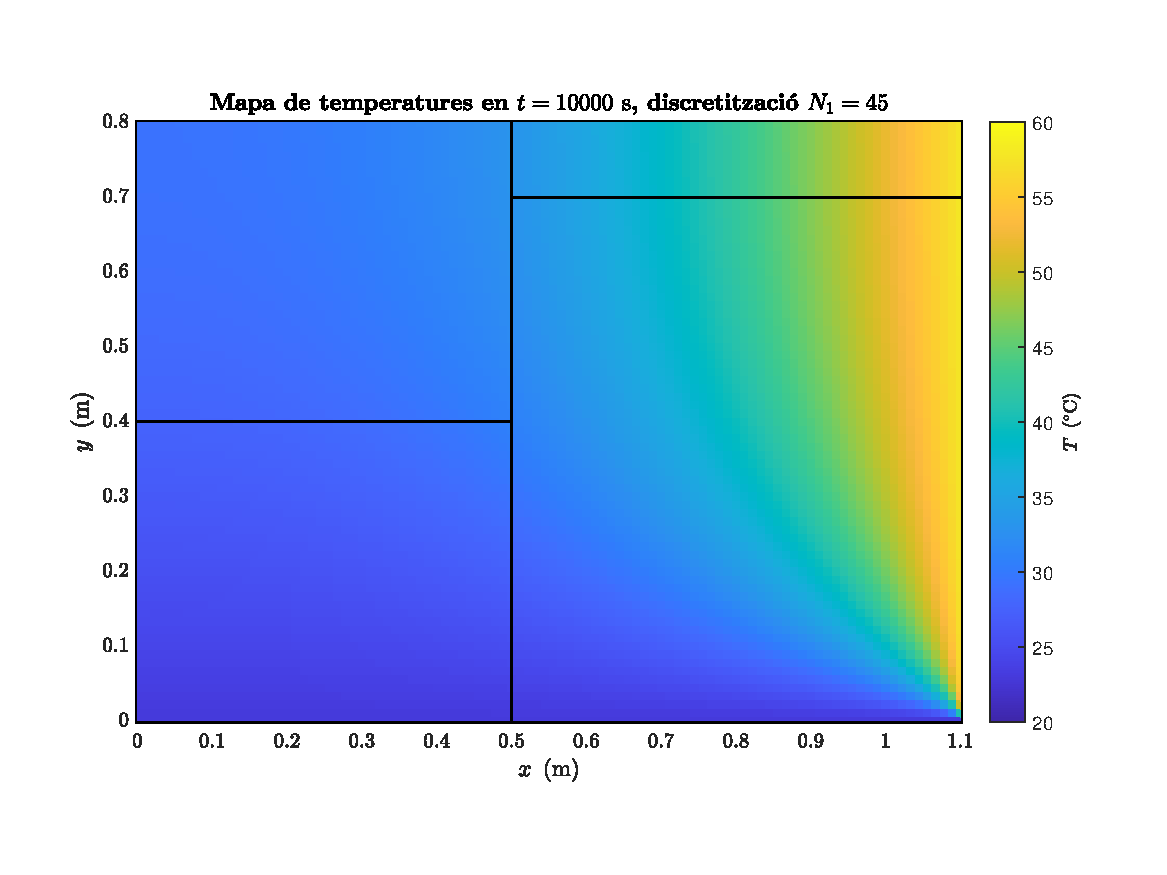
\includegraphics[width=.95\linewidth]{imagenes/04_analisi_influencia_dades_numeriques/malla/malla_11.pdf}
		\vspace{-15pt}
		\caption{Temps $t_\text{max} = 10000 \ \second$, discretització $N_1 = 45$.}
		\label{fig:malla_11}
	\end{subfigure}%
	\begin{subfigure}{.5\textwidth}
		\centering
		\includegraphics[width=.95\linewidth]{imagenes/04_analisi_influencia_dades_numeriques/malla/malla_12.pdf}
		\vspace{-15pt}
		\caption{Temps $t_\text{max} = 10000 \ \second$, discretització $N_1 = 55$.}
		\label{fig:malla_12}
	\end{subfigure}
	\caption{(Anàlisi de la densitat de malla) Mapes de temperatures en $t_\text{max} = 10000 \ \second$, discretitzacions uniformes de $N_1 = 5, \, 15, \, 25, \, 35, \, 45$ i $55$ nodes, pas de temps $\Delta = 1.00 \ \second$, esquema Crank--Nicolson i sense interpolació. L'escala de temperatures és entre $20 \ \celsius$ i $60 \ \celsius$. Els mateixos comentaris fets per $t_\text{max} = 5000 \ \second$ són aplicables al cas actual.}
	\label{fig:malla_10000}
\end{figure} 

%\subsubsection{Pas de temps}

\begin{figure}[ht]
	\centering
	\begin{subfigure}{.5\textwidth}
		\centering
		\includegraphics[width=.95\linewidth]{imagenes/04_analisi_influencia_dades_numeriques/pas_temps/pas_temps_7.pdf}
		\vspace{-15pt}
		\caption{Temps $t_\text{max} = 5000 \ \second$, pas de temps $\Delta t = 0.50 \ \second$.}
		\label{fig:pas_temps_7}
	\end{subfigure}%
	\begin{subfigure}{.5\textwidth}
		\centering
		\includegraphics[width=.95\linewidth]{imagenes/04_analisi_influencia_dades_numeriques/pas_temps/pas_temps_8.pdf}
		\vspace{-15pt}
		\caption{Temps $t_\text{max} = 5000 \ \second$, pas de temps $\Delta t = 1.00 \ \second$.}
		\label{fig:pas_temps_8}
	\end{subfigure}
	\begin{subfigure}{.5\textwidth}
		\centering
		\includegraphics[width=.95\linewidth]{imagenes/04_analisi_influencia_dades_numeriques/pas_temps/pas_temps_9.pdf}
		\vspace{-15pt}
		\caption{Temps $t_\text{max} = 5000 \ \second$, pas de temps $\Delta t = 5.00 \ \second$.}
		\label{fig:pas_temps_9}
	\end{subfigure}%
	\begin{subfigure}{.5\textwidth}
		\centering
		\includegraphics[width=.95\linewidth]{imagenes/04_analisi_influencia_dades_numeriques/pas_temps/pas_temps_10.pdf}
		\vspace{-15pt}
		\caption{Temps $t_\text{max} = 5000 \ \second$, pas de temps $\Delta t = 10.00 \ \second$.}
		\label{fig:pas_temps_10}
	\end{subfigure}
	\begin{subfigure}{.5\textwidth}
		\centering
		\includegraphics[width=.95\linewidth]{imagenes/04_analisi_influencia_dades_numeriques/pas_temps/pas_temps_11.pdf}
		\vspace{-15pt}
		\caption{Temps $t_\text{max} = 5000 \ \second$, pas de temps $\Delta t = 20.00 \ \second$.}
		\label{fig:pas_temps_11}
	\end{subfigure}%
	\begin{subfigure}{.5\textwidth}
		\centering
		\includegraphics[width=.95\linewidth]{imagenes/04_analisi_influencia_dades_numeriques/pas_temps/pas_temps_12.pdf}
		\vspace{-15pt}
		\caption{Temps $t_\text{max} = 5000 \ \second$, pas de temps $\Delta t = 50.00 \ \second$.}
		\label{Temps fig:pas_temps_12}
	\end{subfigure}
	\caption{(Anàlisi del pas de temps) Mapes de temperatures en $t_\text{max} = 5000 \ \second$, discretització uniforme de $N_1 = 35$, amb passos de temps $\Delta = 0.50 \ \second, \, 1.00 \ \second, \, 5.00 \ \second, \, 10.00 \ \second, \, 20.00 \ \second$ i $50.00 \ \second,$, esquema de Crank--Nicolson i sense interpolació. L'escala de temperatures és entre $20 \ \celsius$ i $40 \ \celsius$. Com més petit és $\Delta t$, s'aprecia que la zona de major gradient tèrmic és més àmplia. A mida que $\Delta t$ creix, aquesta zona es retrau cap a la paret dreta. Més enllà d'això, no s'observen diferències significatives que indiquin que per $\Delta t = 0.50 \ \second$ s'obtinguin millors resultats que per $\Delta t = 50.00 \ \second$. Aquest fet té dues justificacions. D'una banda, l'esquema d'integració temporal és de segon ordre. D'altra banda, les propietats termofísiques i les condicions de contorn. Unes conductivitats tèrmiques més grans (\eg, $\lambda \approx 380 \ \watt / \meter \kelvin$ per l'alumini) i uns calors específics més petits, afavoririen la transferència de calor, fent necessari $\Delta t$ més petits.}	
	\label{fig:pas_temps_5000}
\end{figure} 

\begin{figure}[ht]
	\centering
	\begin{subfigure}{.5\textwidth}
		\centering
		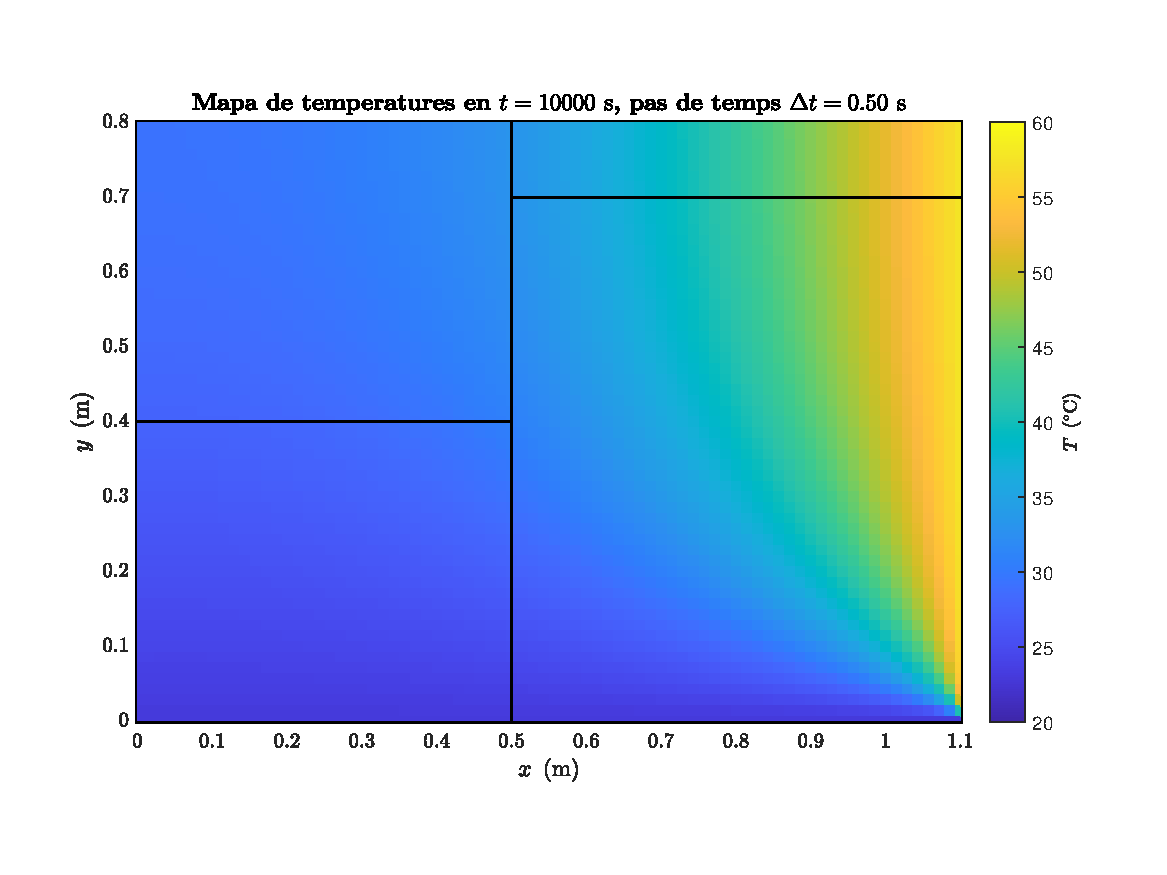
\includegraphics[width=.95\linewidth]{imagenes/04_analisi_influencia_dades_numeriques/pas_temps/pas_temps_13.pdf}
		\vspace{-15pt}
		\caption{Temps $t_\text{max} = 10000 \ \second$, pas de temps $\Delta t = 0.50 \ \second$.}
		\label{fig:pas_temps_13}
	\end{subfigure}%
	\begin{subfigure}{.5\textwidth}
		\centering
		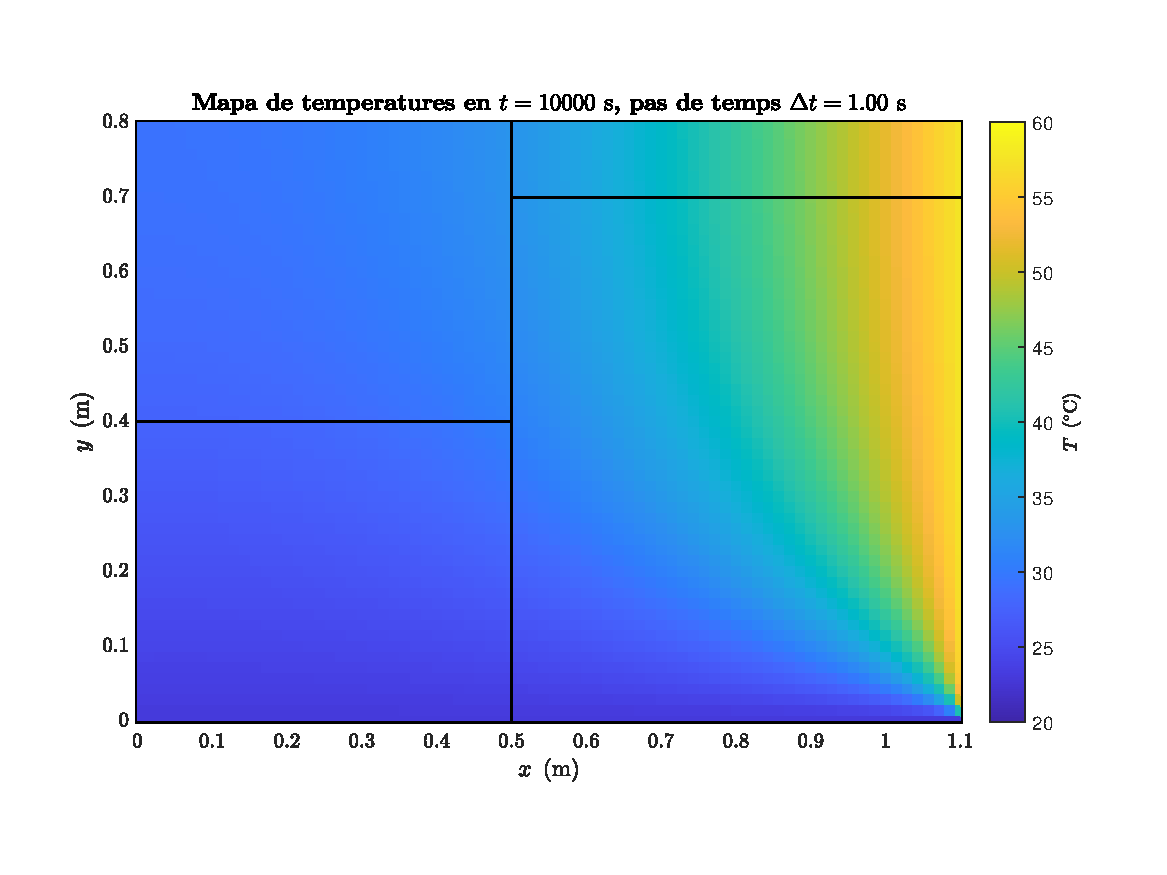
\includegraphics[width=.95\linewidth]{imagenes/04_analisi_influencia_dades_numeriques/pas_temps/pas_temps_14.pdf}
		\vspace{-15pt}
		\caption{Temps $t_\text{max} = 10000 \ \second$, pas de temps $\Delta t = 1.00 \ \second$.}
		\label{fig:pas_temps_14}
	\end{subfigure}
	\begin{subfigure}{.5\textwidth}
		\centering
		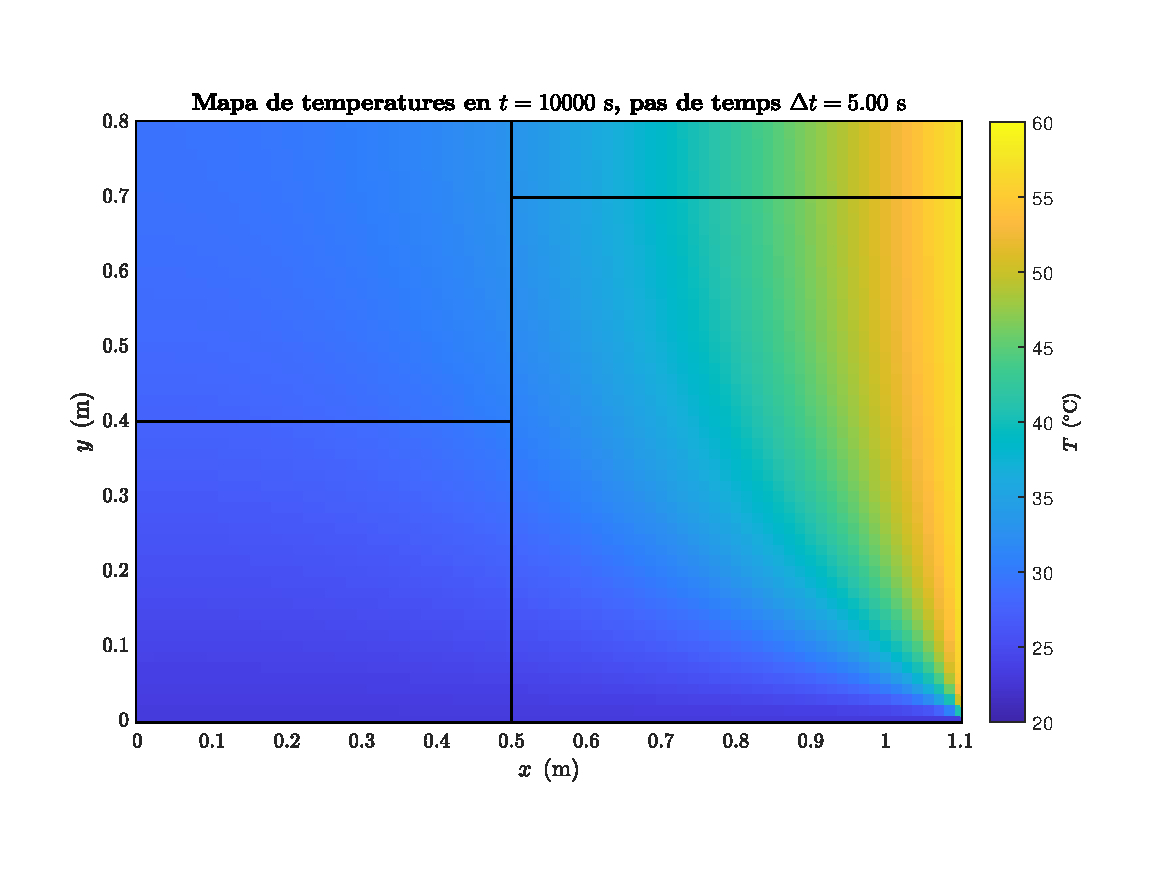
\includegraphics[width=.95\linewidth]{imagenes/04_analisi_influencia_dades_numeriques/pas_temps/pas_temps_15.pdf}
		\vspace{-15pt}
		\caption{Temps $t_\text{max} = 10000 \ \second$, pas de temps $\Delta t = 5.00 \ \second$.}
		\label{fig:pas_temps_15}
	\end{subfigure}%
	\begin{subfigure}{.5\textwidth}
		\centering
		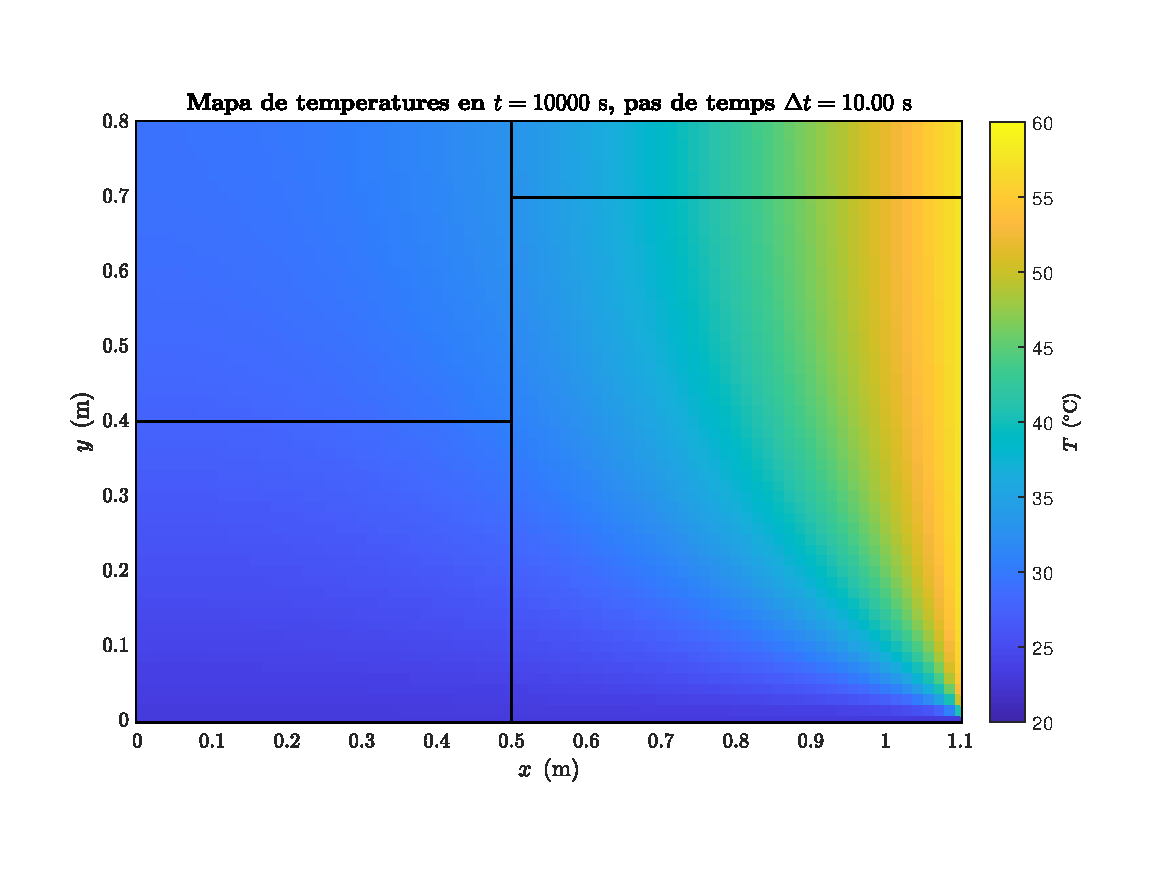
\includegraphics[width=.95\linewidth]{imagenes/04_analisi_influencia_dades_numeriques/pas_temps/pas_temps_16.pdf}
		\vspace{-15pt}
		\caption{Temps $t_\text{max} = 10000 \ \second$, pas de temps $\Delta t = 10.00 \ \second$.}
		\label{fig:pas_temps_16}
	\end{subfigure}
	\begin{subfigure}{.5\textwidth}
		\centering
		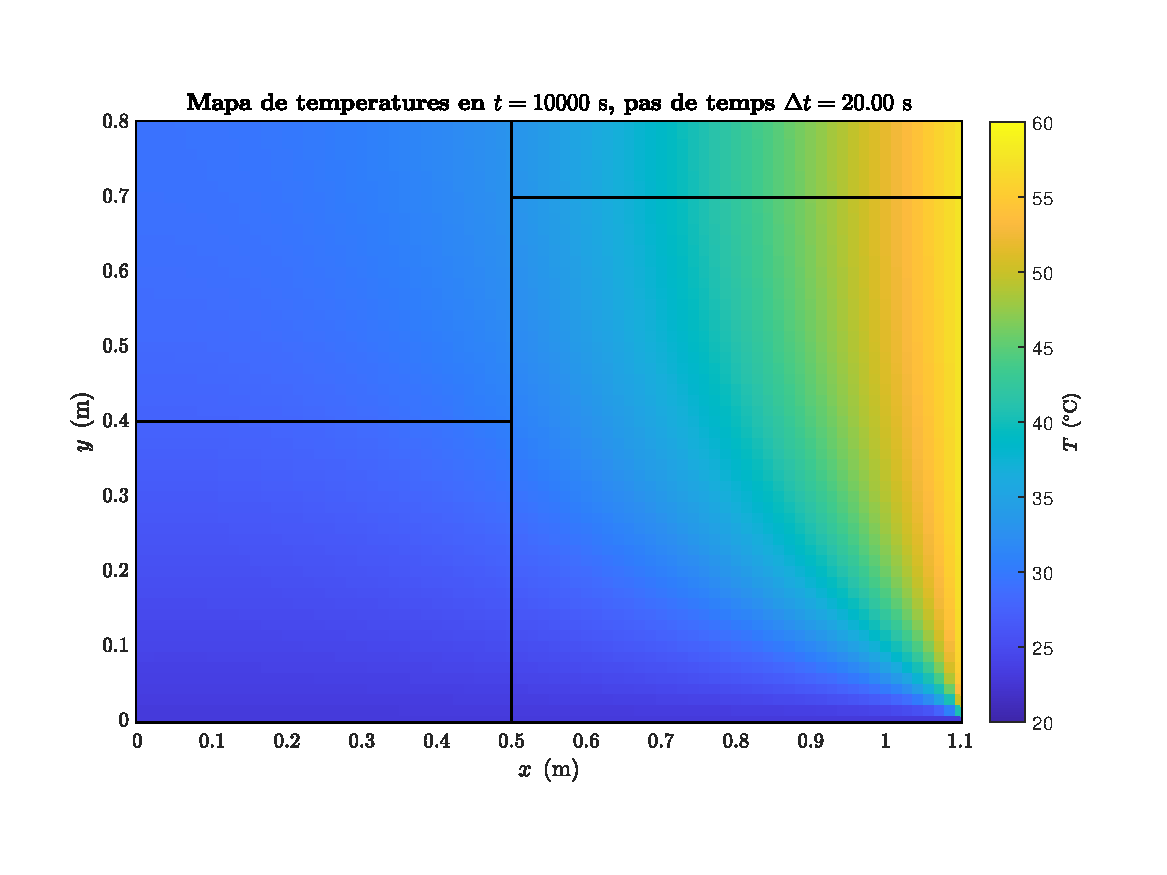
\includegraphics[width=.95\linewidth]{imagenes/04_analisi_influencia_dades_numeriques/pas_temps/pas_temps_17.pdf}
		\vspace{-15pt}
		\caption{Temps $t_\text{max} = 10000 \ \second$, pas de temps $\Delta t = 20.00 \ \second$.}
		\label{fig:pas_temps_17}
	\end{subfigure}%
	\begin{subfigure}{.5\textwidth}
		\centering
		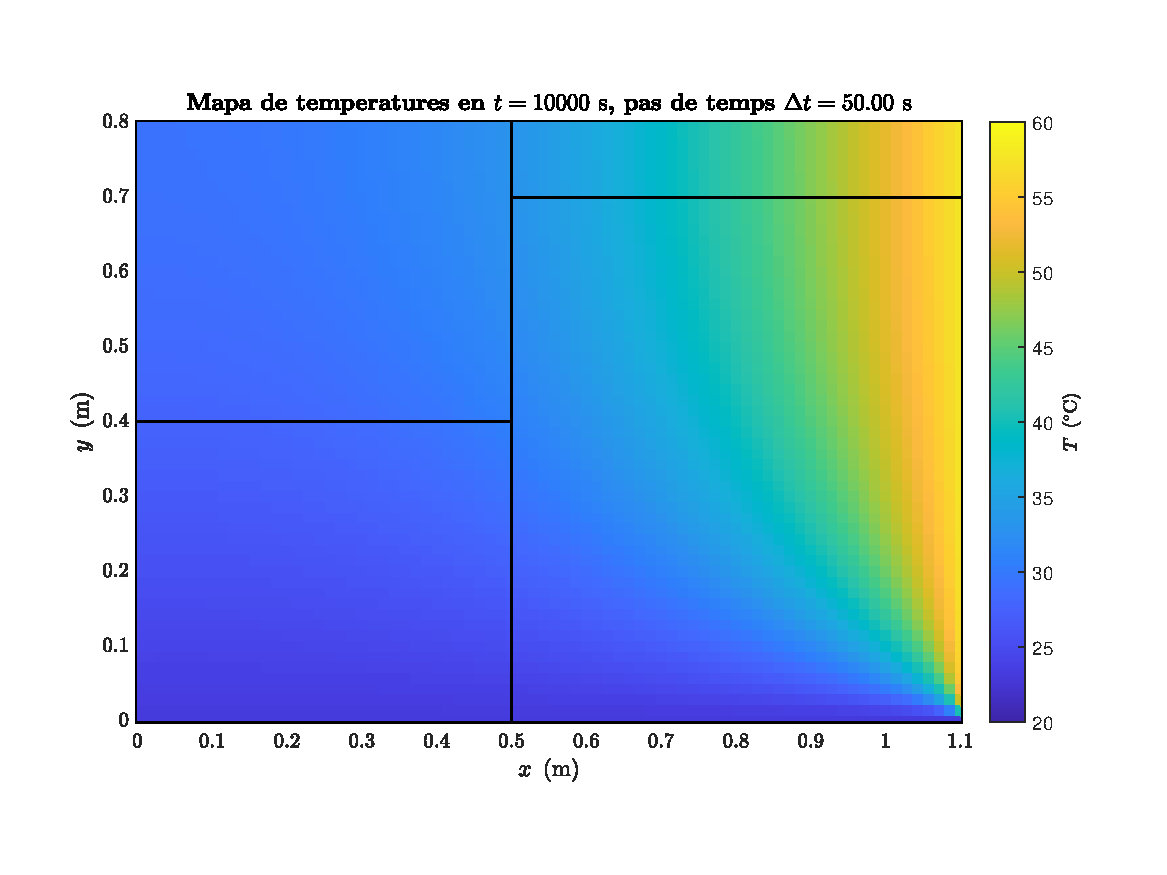
\includegraphics[width=.95\linewidth]{imagenes/04_analisi_influencia_dades_numeriques/pas_temps/pas_temps_18.pdf}
		\vspace{-15pt}
		\caption{Temps $t_\text{max} = 10000 \ \second$, pas de temps $\Delta t = 50.00 \ \second$.}
		\label{Temps fig:pas_temps_18}
	\end{subfigure}
	\caption{(Anàlisi del pas de temps) Mapes de temperatures en $t_\text{max} = 10000 \ \second$, discretització uniforme de $N_1 = 35$, amb passos de temps $\Delta = 0.50 \ \second, \, 1.00 \ \second, \, 5.00 \ \second, \, 10.00 \ \second, \, 20.00 \ \second$ i $50.00 \ \second,$, esquema de Crank--Nicolson i sense interpolació. L'escala de temperatures és entre $20 \ \celsius$ i $60 \ \celsius$. De nou s'observa que la zona de major gradient tèrmic és lleugerament més amplia amb $\Delta t$ petit. Els comentaris anteriors són aplicables en aquest cas.}	
	\label{fig:pas_temps_10000}
\end{figure} 

%\subsubsection{Esquema d'integracio}

\begin{figure}[ht]
	\centering
	\begin{subfigure}{.5\textwidth}
		\centering
		\includegraphics[width=.95\linewidth]{imagenes/04_analisi_influencia_dades_numeriques/esquema/esquema_1.pdf}
		\vspace{-15pt}
		\caption{$t_\text{max} = 5000 \ \second$, $\Delta t = 10.00 \ \second$, implícit.}
		\label{fig:esquema_1}
	\end{subfigure}%
	\begin{subfigure}{.5\textwidth}
		\centering
		\includegraphics[width=.95\linewidth]{imagenes/04_analisi_influencia_dades_numeriques/esquema/esquema_2.pdf}
		\vspace{-15pt}
		\caption{$t_\text{max} = 5000 \ \second$, $\Delta t = 10.00 \ \second$, Crank--Nicolson.}
		\label{fig:esquema_2}
	\end{subfigure}
	\begin{subfigure}{.5\textwidth}
		\centering
		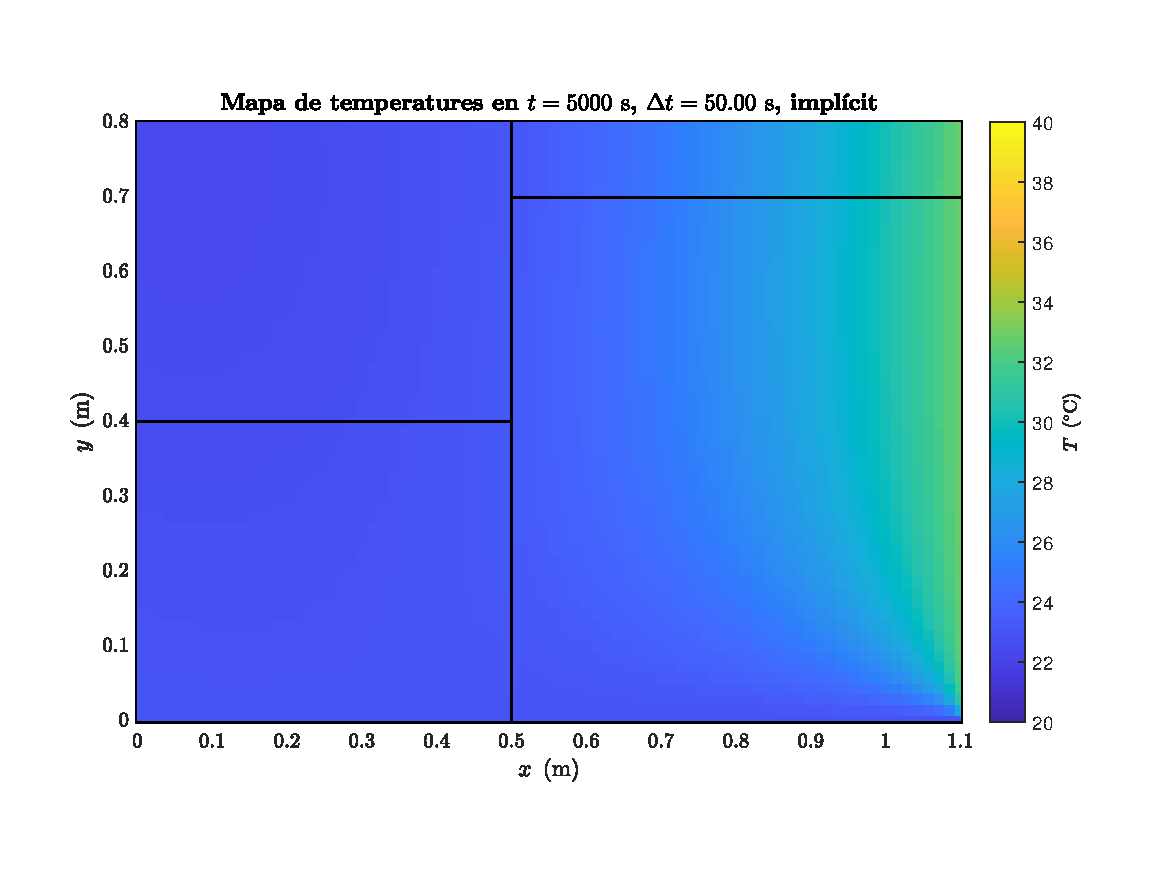
\includegraphics[width=.95\linewidth]{imagenes/04_analisi_influencia_dades_numeriques/esquema/esquema_3.pdf}
		\vspace{-15pt}
		\caption{$t_\text{max} = 5000 \ \second$, $\Delta t = 50.00 \ \second$, implícit.}
		\label{fig:esquema_3}
	\end{subfigure}%
	\begin{subfigure}{.5\textwidth}
		\centering
		\includegraphics[width=.95\linewidth]{imagenes/04_analisi_influencia_dades_numeriques/esquema/esquema_4.pdf}
		\vspace{-15pt}
		\caption{$t_\text{max} = 5000 \ \second$, $\Delta t = 50.00 \ \second$, Crank--Nicolson.}
		\label{fig:esquema_4}
	\end{subfigure}
	\begin{subfigure}{.5\textwidth}
		\centering
		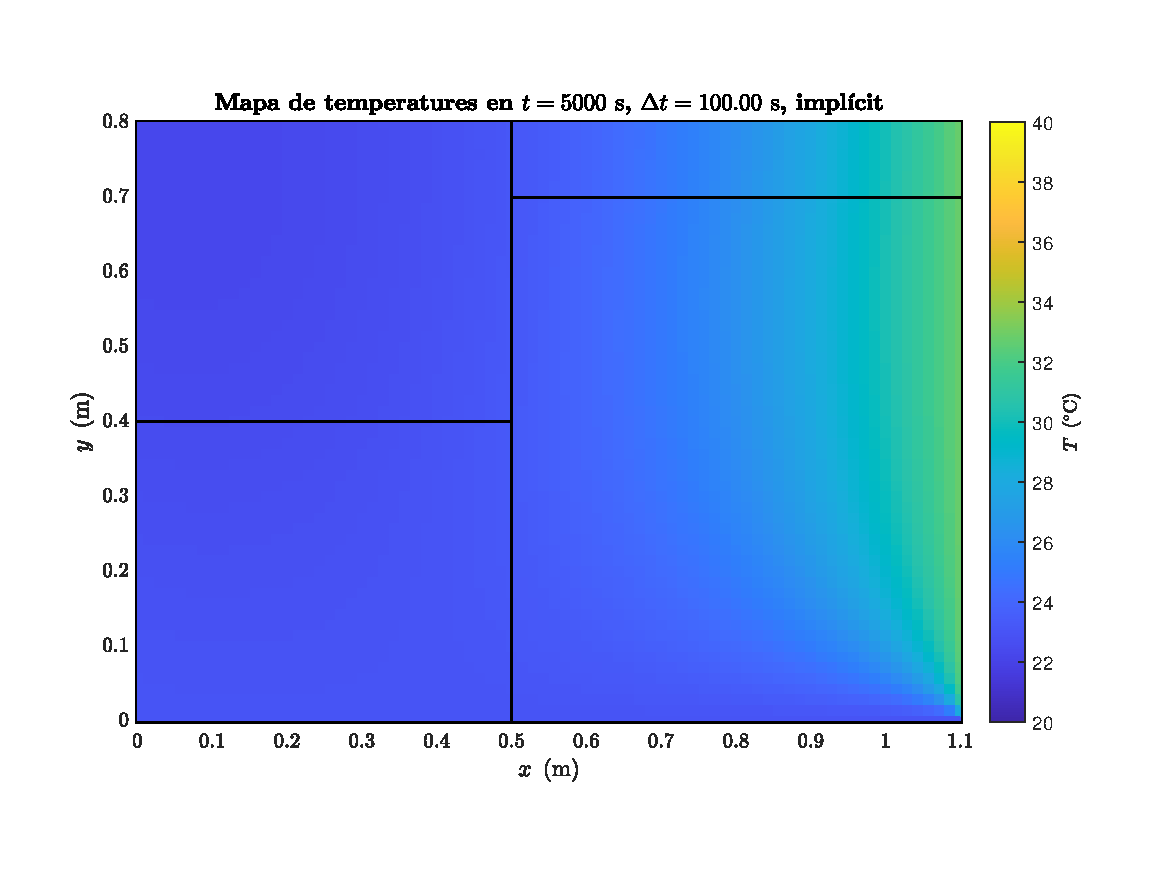
\includegraphics[width=.95\linewidth]{imagenes/04_analisi_influencia_dades_numeriques/esquema/esquema_5.pdf}
		\vspace{-15pt}
		\caption{$t_\text{max} = 5000 \ \second$, $\Delta t = 100.00 \ \second$, implícit.}
		\label{fig:esquema_5}
	\end{subfigure}%
	\begin{subfigure}{.5\textwidth}
		\centering
		\includegraphics[width=.95\linewidth]{imagenes/04_analisi_influencia_dades_numeriques/esquema/esquema_6.pdf}
		\vspace{-15pt}
		\caption{$t_\text{max} = 5000 \ \second$, $\Delta t = 100.00 \ \second$, Crank--Nicolson.}
		\label{fig:esquema_6}
	\end{subfigure}
	\caption{(Anàlisi de l'esquema d'integració) Mapes de temperatures en $t_\text{max} = 5000 \ \second$, amb discretització uniforme de $N_1 = 35$, passos de temps $\Delta t = 10.00 \ \second$, $50.00 \ \second$ i $100.00 \ \second$, sense interpolació. L'escala de temperatures és entre $20 \ \celsius$ i $40 \ \celsius$. Els esquemes implícits es troben a la columna esquerre i els esquemes de Crank--Nicolson a la columna dreta. No s'observen diferències significatives entre els esquemes d'integració per $\Delta t = 10.00 \ \second$ i $\Delta t = 50.00 \ \second$. Tanmateix, en l'esquema de Crank--Nicolson, per $\Delta t = 100.00 \ \second$, s'aprecia una franja horizontal de baixa temperatura en la part inferior del domini que, aparentment, no guarda relació amb la realitat física. Aquesta mateixa franja no apareix en l'esquema implícit.}	
	\label{fig:esquema_5000}
\end{figure} 

\begin{figure}[ht]
	\centering
	\begin{subfigure}{.5\textwidth}
		\centering
		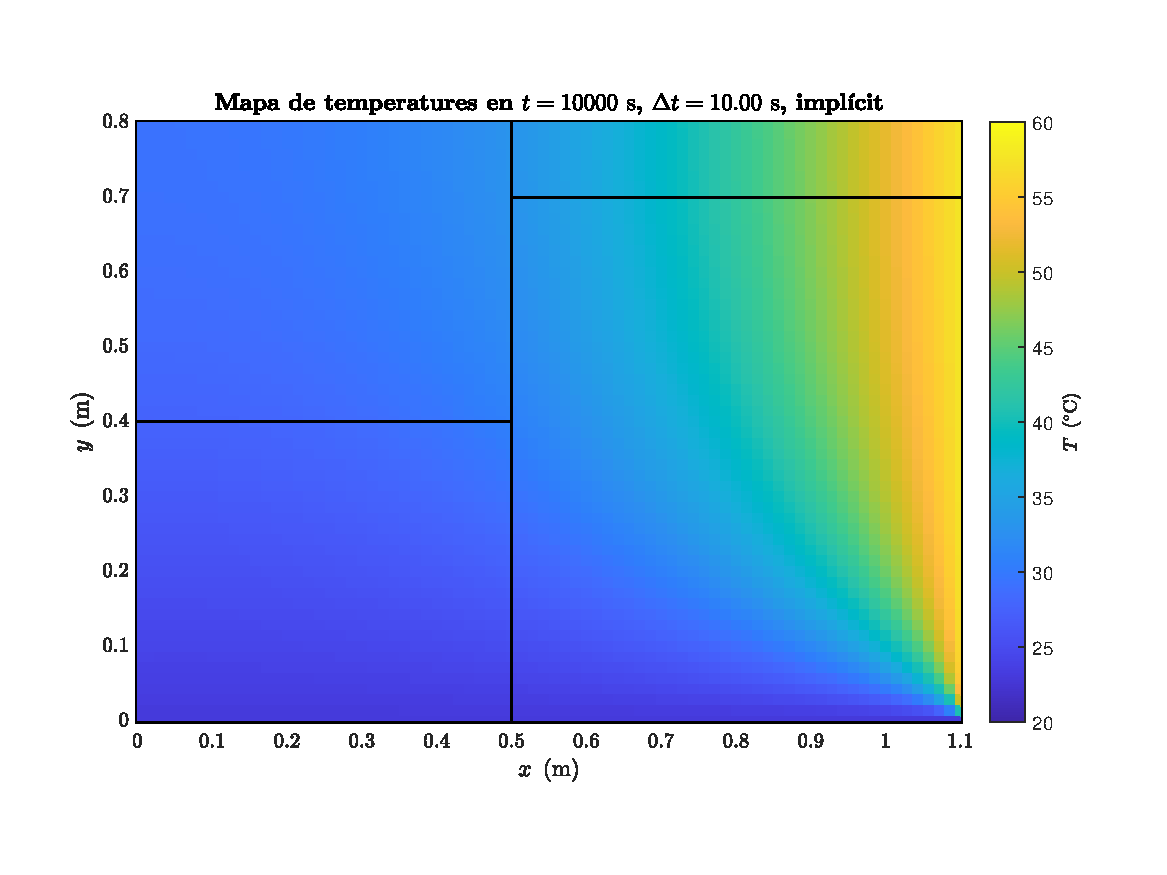
\includegraphics[width=.95\linewidth]{imagenes/04_analisi_influencia_dades_numeriques/esquema/esquema_7.pdf}
		\vspace{-15pt}
		\caption{$t_\text{max} = 10000 \ \second$, $\Delta t = 10.00 \ \second$, implícit.}
		\label{fig:esquema_7}
	\end{subfigure}%
	\begin{subfigure}{.5\textwidth}
		\centering
		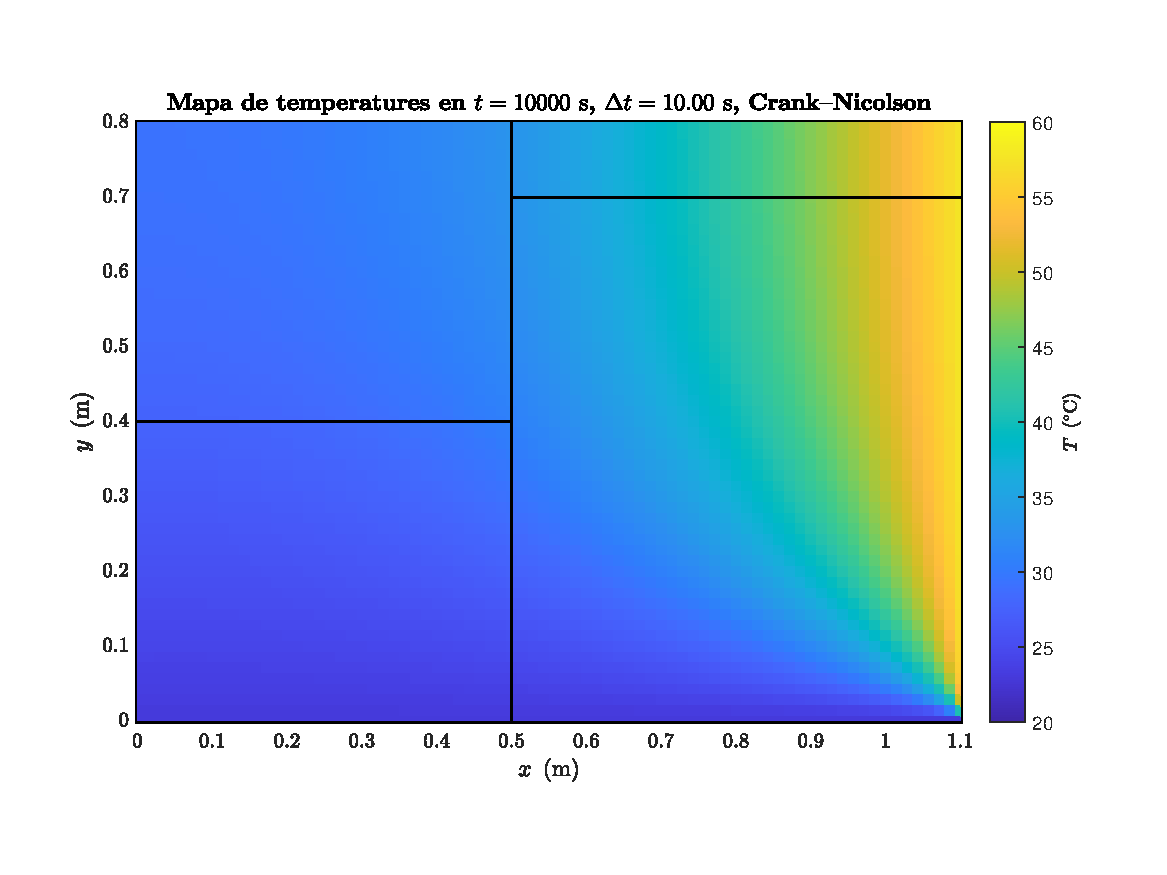
\includegraphics[width=.95\linewidth]{imagenes/04_analisi_influencia_dades_numeriques/esquema/esquema_8.pdf}
		\vspace{-15pt}
		\caption{$t_\text{max} = 10000 \ \second$, $\Delta t = 10.00 \ \second$, Crank--Nicolson.}
		\label{fig:esquema_8}
	\end{subfigure}
	\begin{subfigure}{.5\textwidth}
		\centering
		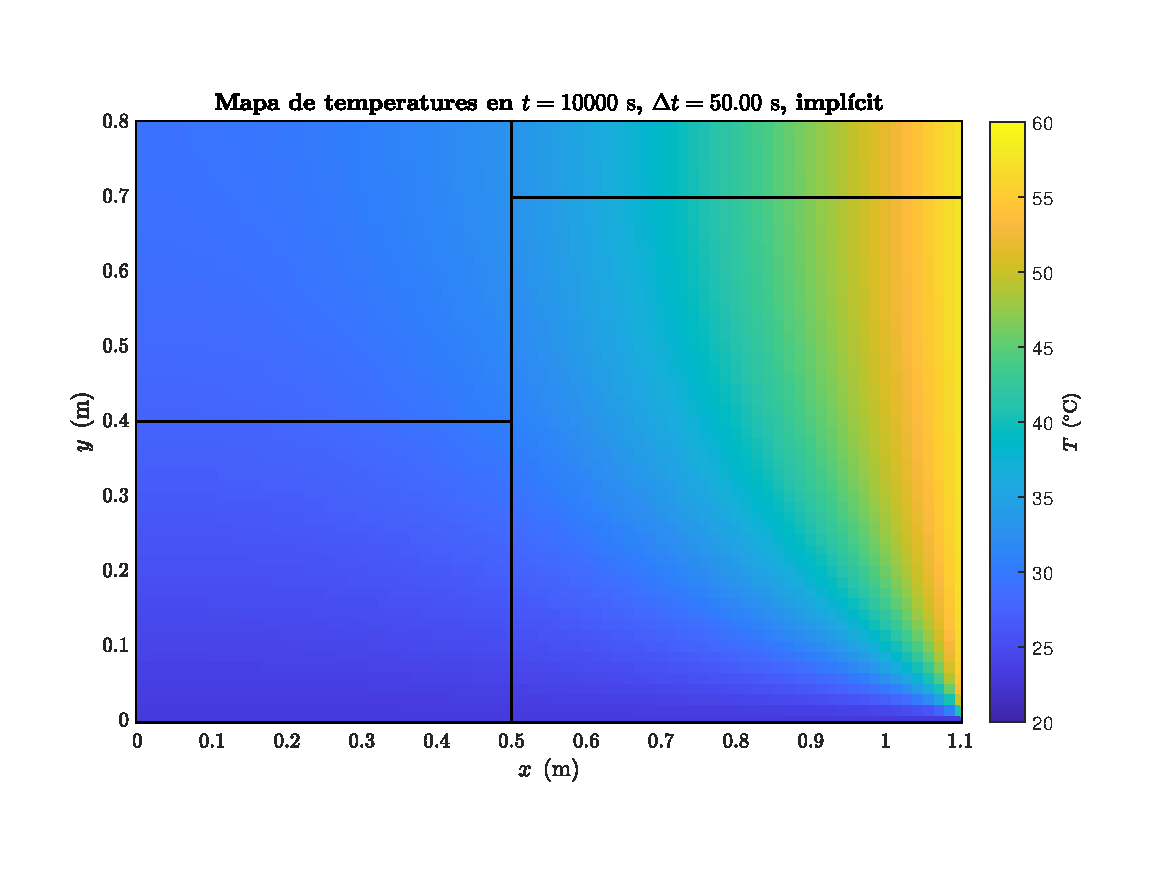
\includegraphics[width=.95\linewidth]{imagenes/04_analisi_influencia_dades_numeriques/esquema/esquema_9.pdf}
		\vspace{-15pt}
		\caption{$t_\text{max} = 10000 \ \second$, $\Delta t = 50.00 \ \second$, implícit.}
		\label{fig:esquema_9}
	\end{subfigure}%
	\begin{subfigure}{.5\textwidth}
		\centering
		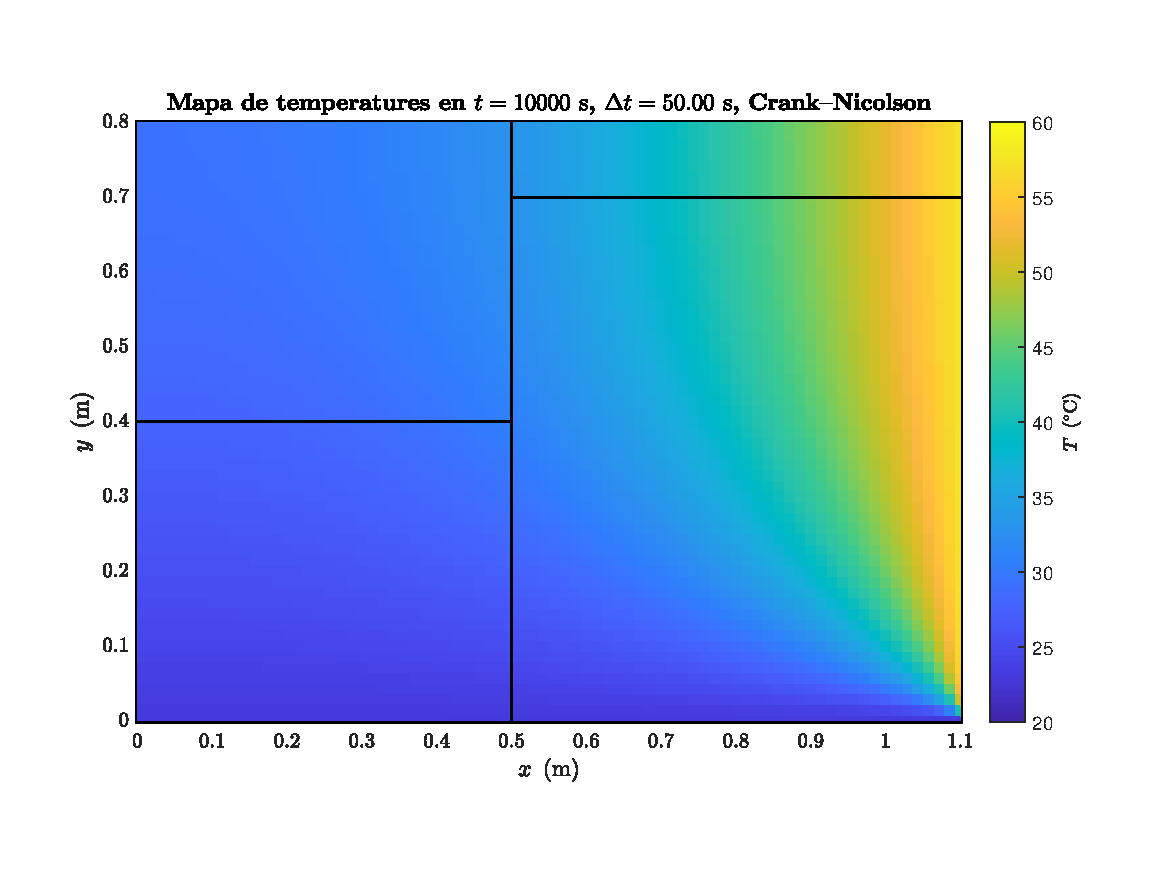
\includegraphics[width=.95\linewidth]{imagenes/04_analisi_influencia_dades_numeriques/esquema/esquema_10.pdf}
		\vspace{-15pt}
		\caption{$t_\text{max} = 10000 \ \second$, $\Delta t = 50.00 \ \second$, Crank--Nicolson.}
		\label{fig:esquema_10}
	\end{subfigure}
	\begin{subfigure}{.5\textwidth}
		\centering
		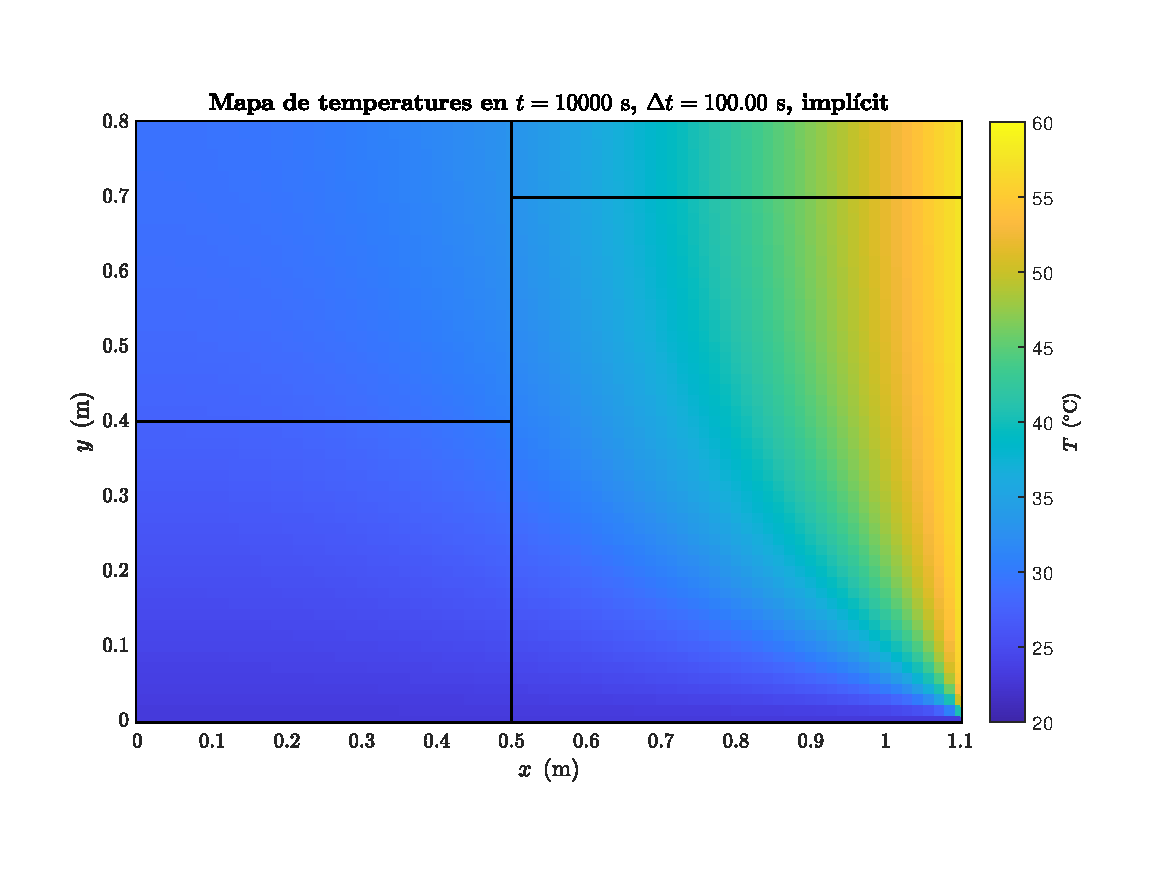
\includegraphics[width=.95\linewidth]{imagenes/04_analisi_influencia_dades_numeriques/esquema/esquema_11.pdf}
		\vspace{-15pt}
		\caption{$t_\text{max} = 10000 \ \second$, $\Delta t = 100.00 \ \second$, implícit.}
		\label{fig:esquema_11}
	\end{subfigure}%
	\begin{subfigure}{.5\textwidth}
		\centering
		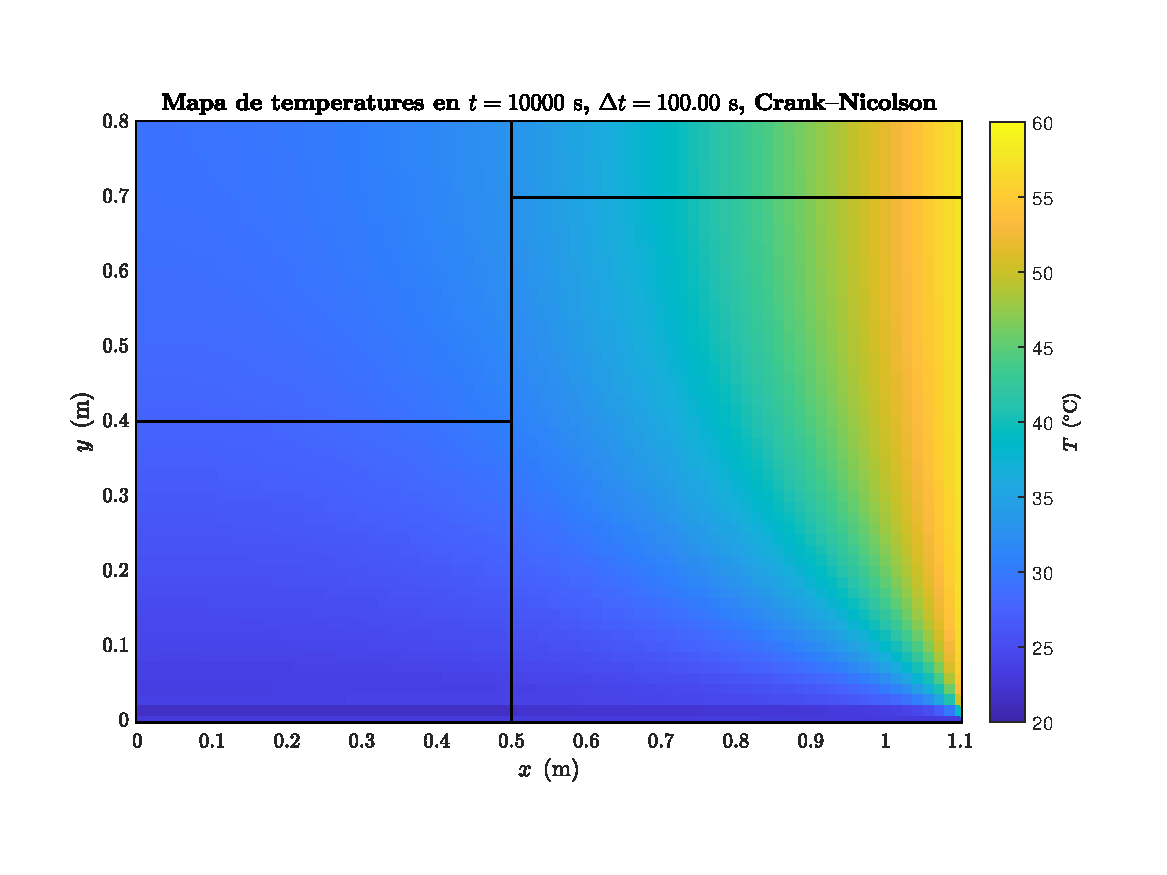
\includegraphics[width=.95\linewidth]{imagenes/04_analisi_influencia_dades_numeriques/esquema/esquema_12.pdf}
		\vspace{-15pt}
		\caption{$t_\text{max} = 10000 \ \second$, $\Delta t = 100.00 \ \second$, Crank--Nicolson.}
		\label{fig:esquema_12}
	\end{subfigure}
	\caption{(Anàlisi de l'esquema d'integració) Mapes de temperatures en $t_\text{max} = 10000 \ \second$, amb discretització uniforme de $N_1 = 35$, passos de temps $\Delta t = 10.00 \ \second$, $50.00 \ \second$ i $100.00 \ \second$, sense interpolació. L'escala de temperatures és entre $20 \ \celsius$ i $60 \ \celsius$. D'igual manera que en el cas anterior, no s'observen diferències significatives entre els esquemes d'integració per $\Delta t = 10.00 \ \second$ i $\Delta t = 50.00 \ \second$. Per l'esquema de Crank--Nicolson i $\Delta t = 100.00 \ \second$, la franja de baixa temperatura en persisteix.}		
	\label{fig:esquema_10000}
\end{figure} 